\section{Introduzione}
Ricordiamo cosa può essere protetto dal diritto di proprietà intellettuale.\bigskip
I brevetti costituiscono una buona parte della proprietà intellettuale: i brevetti sono sulle nuove invenzioni e vengono garantiti attraverso una richiesta a cui fa seguito un'esaminazione.
Al contrario, gli Utility models (modello di utilità) costituiscono una sotto-famiglia dei brevetti che hanno costi inferiori e un iter più breve per il rilascio.
Infine il copyright esiste automaticamente alla creazione dell'opera (poi l'autore ne collezionerà una prova o autenticazione).

Altre categorie importanti sono: 
\begin{itemize}
    \item Trade marks: distinzione identificativa di prodotti o servizi; si ottiene tramite registrazione.
    \item Design registrati: proteggono un'apparenza esteriore/estetica (es. la forma della bottiglia della \textit{Coca-Cola}); si ottiene tramite registrazione.
    \item Trade secrets (segreti industriali): si usa per proteggere informazioni di valore che non devono essere divulgate; si mantiene il segreto tramite sforzi che dipendono dalla singola azienda
\end{itemize}

Queste forme di proprietà intellettuale possono essere combinate tra loro, come mostrato in figura \ref{IP rights}. 

\begin{figure}
    \centering
    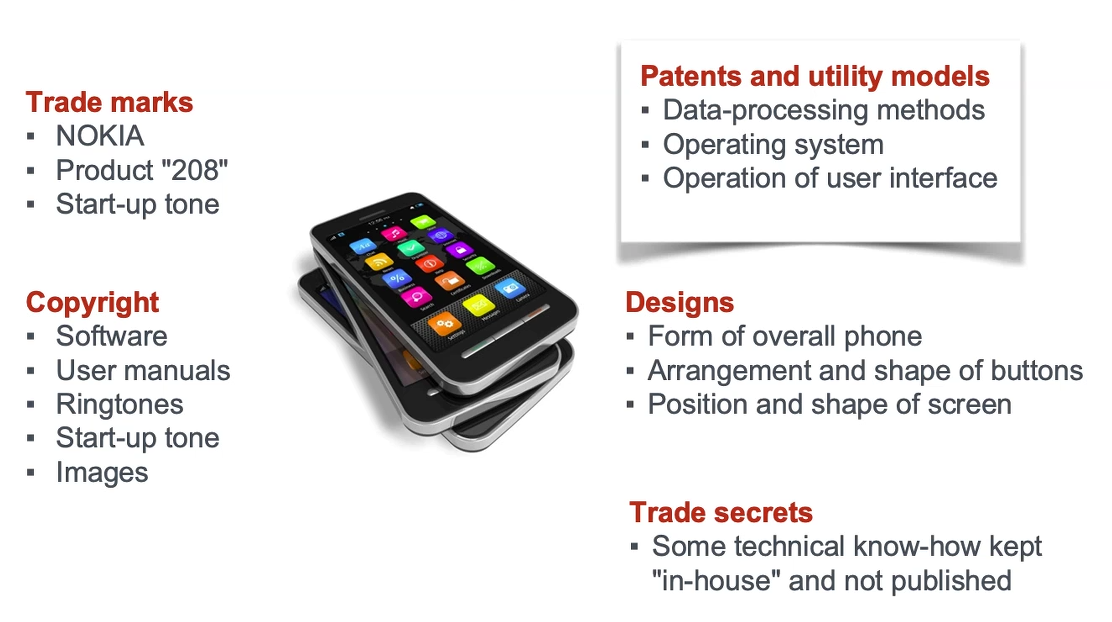
\includegraphics[width=\textwidth]{IP rights.png}
    \caption{Combinazione di più diritti di proprietà intellettuale}
    \label{IP rights}
\end{figure}

Il sistema di brevetti promuove:
\begin{itemize}
    \item L'innovazione tecnologica
    \item La competizione e l'investimento
    \item La fornitura di informazioni relative agli avanzamenti tecnologici più recenti
    \item La diffusione della tecnologia
\end{itemize}

\subsection{Storia dei brevetti}
I brevetti nascono nell'Antica Grecia, nel V secolo a.C., per poi essere ridefinito durante il periodo di dominazione Veneta sul Mediterraneo, in particolare nel 1474.

\begin{figure}
    \centering
    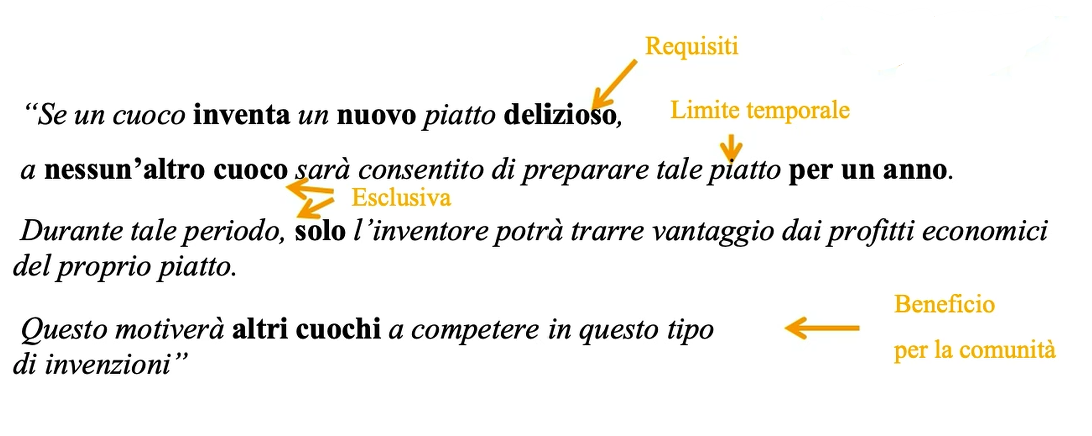
\includegraphics{nascita brevetto.png}
    \caption{Prima definizione di brevetto - Magna Grecia}
\end{figure}

\subsection{Natura giuridica del brevetto}
Il brevetto è uno strumento di riconoscimento attuato dallo Stato al fine di riconoscere l'inventore di un determinato prodotto.\bigskip

Una volta che viene concesso un brevetto, non si è automaticamente autorizzati a produrre il bene brevettato: ciò che si ha è il diritto di escludere terzi dallo sfruttare tale invenzione. 

Avere un'esclusiva su un'invenzione consiste nell'autorizzazione da parte della legge ad essere monopolisti relativamente all'invenzione; allo scadere del brevetto l'invenzione diventa di pubblico dominio.

Il monopolio temporaneo ha durata quasi ovunque fissata in 20 anni dal deposito della domanda di brevetto.\bigskip

ATTENZIONE: se non viene brevettata un'invenzione, essa potrebbe venire brevettata da qualcun altro, i competitori potrebbero trarne vantaggio oppure si potranno in futuro verificare situazioni in cui la vendita del prodotto sia minata dall'assenza di brevetto. 

\subsection{Vantaggi e svantaggi dei brevetti}
\begin{table}[h]
    \centering
    \begin{tabular}{|p{6.5cm}|p{6.5cm}|}
        \hline
        Vantaggi & Svantaggi \\
        \hline
        \begin{itemize}
            \item L'esclusività garantisce la possibilità di investimenti e maggiori ritorni di investimento
            \item Diritti legali
            \item Rende l'invenzione commercializzabile (tramite licenza o vendita)
        \end{itemize} & \begin{itemize}
            \item Rivela l'invenzione ai competitori dopo 18 mesi 
            \item Può essere costoso
            \item La concessione può avvenire dopo 3-5 anni dalla domanda
        \end{itemize}\\
        \hline
    \end{tabular}
    \caption{Vantaggi e svantaggi dell'uso dei brevetti}
\end{table}

\subsection{Alternative al brevetto}
Un meccanismo interessante è quello di rendere pubblica la propria invenzione senza brevettarla: si tratta di un meccanismo gratuito e impedisce a terzi di brevettare la stessa invenzione (si può brevettare solo qualcosa che non è ancora esistente/conosciuto, quindi se qualcosa è di dominio pubblico è già esistente e non più brevettabile). 

Chiaramente in questo modo non si ha l'esclusiva sull'invenzione.\bigskip

Un'alternativa ulteriore è il rivelare solo parte della propria invenzione a terzi. \bigskip

Inoltre si può mantenere il segreto sull'invenzione (gratuito a meno di tecniche di mantenimento del segreto - impianti di allarme, etc.). Si tratta di un metodo utile quando dall'invenzione non si può effettuare reverse engineering.\bigskip

L'ultimo metodo consiste nel non far niente, ma chiaramente non garantisce l'esclusività sul possesso dell'invenzione e spesso i competitori possono apprendere numerosi dettagli sull'invenzione.
